\documentclass[11pt]{article}
\usepackage{../ee16}
\usepackage{../markup}
\usepackage{changepage}
\usepackage{tikz}
\usetikzlibrary{calc}
\usepackage{color,hyperref,listings,enumitem}
\usepackage{algorithm}
\usepackage{algpseudocode}
\usepackage{tkz-euclide}
\usepackage{physics}
\usepackage{multicol}
\usepackage{pgfplots}
\usepackage{adjustbox}
\usepackage{cancel}
\usepackage{commath}
\usepackage{graphicx}
\usepackage{mathdots}
\usepackage{subcaption}
\usepackage[american,siunitx]{circuitikz}
\sisetup{per-mode=fraction}
\sisetup{quotient-mode=fraction}
\DeclareSIUnit \decade {dec}
\lstset{basicstyle=\ttfamily}
\newcommand{\fillin}[1]{\underline{\hskip #1}}
\newcommand{\doublehrule}{\hrule \vskip 0.02in \hrule}
\newcommand*\circled[1]{\tikz[baseline=(char.base)]{
  \node[shape=circle,draw,inner sep=2pt] (char) {#1};}}

\definecolor{blueish}{rgb}{0.7,0.1,.7}
\newcommand{\sol}[1]{{\color{blueish} \textbf{Solution: } #1}} % solutions in pink
\newcommand{\ws}[1]{} % worksheet exclusive material
\newcommand{\meta}[1]{} % no meta in solutions

\input{../../newcommands/newcommands-eg-ie-etc}
\input{../../newcommands/newcommands-labels-refs}
\input{../../newcommands/newcommands-math}


\usetikzlibrary{positioning}

\begin{document}

\def\title{Worksheet 3}

\newcommand{\qitem}{\qpart\item}

\renewcommand{\labelenumi}{(\alph{enumi})} % change default enum format to (a)
\renewcommand{\theenumi}{(\alph{enumi})} % fix reference format accordingly.
\renewcommand{\labelenumii}{\roman{enumii}.} % second level labels.
\renewcommand{\theenumii}{\roman{enumii}.}

\maketitle

\vspace{0.5em}

\begin{qunlist}

\qns{Voltage Divider}

% \textbf{Learning Goal:} .

Let's take a systematic look at the voltages across a resistor, and see how other components in the circuit can affect it.
Consider the following circuit:
\begin{center}
    \begin{circuitikz}
    \draw(0,0)
	to[V_=$V$,invert] ++(0,5)
 	to[short] ++(3,0)
	to[short] ++(0,-1)
	to[R,l=$R_1$] ++(0,-1)
	to[short] ++(0,-1)
	to[R,l=$R_2$] ++(0,-1)
	to[short] ++(0,-1)
	to[short] node[]{} ++(-3,0);
    \end{circuitikz}
\end{center}
\meta{This problem is intended to give students a deeper understanding on voltage dividers and how circuits can get loaded. It would help students if mentors went over equivalences of resistors in series and in parallel.}

\begin{enumerate}
\item{
Calculate the voltage drop across $R_1$ and $R_2$ using series resistance calculations.}

\meta{It is important to show students that we can simplify complicated circuits by using equivalence relationships.  Also help students understand why the current through the two resistors would be the same.}

\sol{The current out of the voltage source is given by Ohm's law:
\begin{align*}
    i &= \frac{V}{R_{eq}} \\
    i &= \frac{V}{R_1 + R_2}
\end{align*}
Again, by Ohm's law, we have that
\begin{align*}
V_{R_1} = i R_1 = V \frac{R_1}{R_1 + R_2} \\
V_{R_2} = i R_2 = V \frac{R_2}{R_1 + R_2}
\end{align*}}

\item Suppose we want to manipulate the voltage across $R_2$, but it's locked in a box with the voltage source, as denoted below. Can we use $R_1$ to manipulate $V_{R_2}$? What range of voltages can we achieve? 
\begin{center}
    \begin{circuitikz}[scale=0.8]
    \filldraw[fill=gray!40!white,draw=black] (-1,-0.5) rectangle (4,7.5);
    \draw(0,0)
	to[V_=$V$,invert] ++(0,7)
 	to[short,-o] ++(5,0)
	to[short] ++(0,-1)
	to[R,l=$R_1$] ++(0,-1)
	to[short,-o] ++(0,-1)
	to[short] ++(-2,0)
	to[short] ++(0,-1)
	to[short] ++(1,0)
	to[short,l=$V_{R_2}$,-o] ++(1,0)
	-- ++(-2,0)
	to[short] ++(0,-1)
	to[R,l=$R_2$] ++(0,-1)
	to[short] ++(0,-1)
	to[short,-o] ++(2,0)
	-- ++(-2,0)
	to[short] ++(-3,0)
	to[short] node[ground]{} ++(0,-1);
	
	\end{circuitikz}
\end{center}

\meta{
This section highlights the different properties of voltage dividers and how the voltage drop across one component can be manipulated by the ratio resistors in the voltage divider. 
}

\sol{Any voltage in the range $(0, V]$! Notice from the equations above that $V_{R_2} = V \frac{R_2}{R_{Total}}$. If we increase $R_1$ indefinitely, holding $R_2$ constant, we can make the fraction arbitrarily small. Intuitively, since the same current flows through both $R_1$ and $R_2$, they have to split the total voltage of the power source, and larger resistances correspond to larger voltage drops (by Ohm's Law). If we decrease $R_1$ to $0$, $V_{R_2} = V$, so the voltage can be at most whatever is supplied by the power source. That the voltage source limits the achievable voltage in the circuit is a concept we will see again when we cover clipping in op-amps.}

\item Now let's try using our new variable voltage source to power a light bulb with resistance $R_L$, where the threshold voltage for lighting the bulb is $6 \text{V}$. Find $R_1$ and $R_2$ so that the voltage across $R_2$ is this threshold voltage; that is, $V_{R_2} \equiv V_{out} = 6 \text{V}$. Assume we have a $12 \text{V}$ voltage source.

\begin{center}
    \begin{circuitikz}[scale=0.8]
    \filldraw[fill=gray!40!white,draw=black] (-1,-0.5) rectangle (4,7.5);
    \draw(0,0)
	to[V_=$12 \text{V}$,invert] ++(0,7)
 	to[short,-o] ++(3,0)
	to[short] ++(0,-1)
	to[R,l=$R_1$] ++(0,-1)
	to[short,-o] ++(0,-1)
	to[short] ++(0,-1)
	to[short] ++(1,0)
	to[short,l=$\quad \quad V_{out} \equiv 6\text{V}$,-o] ++(1,0)
	-- ++(-2,0)
	to[short] ++(0,-1)
	to[R,l=$R_2$] ++(0,-1)
	to[short] ++(0,-1)
	to[short,-o] ++(2,0)
	-- ++(-2,0)
	to[short] ++(-3,0)
	to[short] node[ground]{} ++(0,-1);
	
 	\draw(5,3)[dashed] 
 	-- ++(2,0); 
 	\draw(7,3)
 	to[lamp,l=$R_L$] ++(0,-3);
%  	to[R,l=$R_L$] ++(0,-3);
 	\draw(7,0)[dashed]
 	-- ++(-2,0);
	\end{circuitikz}
\end{center}


\meta{
Make sure to point out that the lightbulb is not connected yet and that we need to voltage drop across $R_2$ to be 6 volts.}

\sol{We want to split the voltage in half (from 12 to 6). Based on the voltage divider formula above, that means $R_1 = R_2 \equiv R$. Note that, under this condition, the voltage is evenly split regardless of what the actual resistance values are! While the current depends on actual resistance values, the voltage only depends on the ratio of resistances.}

\item Now that we found an $R_1$ and $R_2$ that seem to divide our voltage source appropriately, let's try to connect the bulb to the ends of $R_2$. Remember, the bulb has a resistance $R_L$. Calculate the voltage across $R_1$, $R_2$ and the light bulb when it is connected. Will the light bulb turn on?

\meta We see that once we add the resistor in parallel with $R_2$ the overall resistance decreases therefore our $V_out$ will decrease as well. It might help to point out this relationship using Ohm’s law: $V = IR$.  This is usually the most difficult section for students to conceptualize so make sure to be very clear in the relationships between different components in a circuit.

\sol{Let's reapply the voltage divider formula, but now notice that the "second" resistor is $R_2 \| V_L$!. When we change the resistance in a voltage divider circuit, the voltage across that resistance changes as well. We find that $V_{R_1} = V \frac{R}{R + R \| R_L} = 12\text{V} \frac{R}{R + \frac{R R_L}{R + R_L}} = 12\text{V} \frac{R + R_L}{R+2 R_L}$. The rest of the potential drop must be across the $R_2$-$R_L$ system, so we have $V_{R_2} = V_{\text{bulb}} = 12\text{V} \left(1 - \frac{R + R_L} {R + 2 R_L}\right) = 12\text{V} \frac{R_L}{R + 2 R_L} \leq 12\text{V} \frac{R_L}{2 R_L} = 6\text{V}$. 


So the voltage \textit{decreased}, and the light bulb doesn't turn on. 


The takeaway from this is that, while it may seem like the voltage divider can make voltage sources of arbitrary voltages, the act of connecting a component actually changes the output of the voltage divider. We will later learn about a way to stop a light bulb (or other devices that use up power) from ``affecting" the circuit that supplies power by placing a ``buffer" between the two.}
\end{enumerate}
\newpage
% Author: Jessica Lin
% Email: jessica.jx.lin@berkeley.edu
% CSM16A Fall 2022

% node[label={[font=\footnotesize]above:$u_1$}] {}

\qns{NVA for a Current Divider}

\textbf{Learning Goal:} The goal of this question is to use NVA to derive the equation of a current divider.

\meta{}

\begin{enumerate}

\item Use NVA to solve for $u_1$, $i_{R_1}$, and $i_{R_2}$ in terms of $I_s$, $R_1$, and $R_2$. 

\begin{center}
\begin{circuitikz} 
\draw (0, 0)
to [isource, i = $I_s$,] (0, 3)
to [short, -*] (2.5, 3) node[label={[font=\footnotesize]:$u_1$}]{}
to [short] (5, 3)
to [R = $R_2$, i = $i_{R_2}$] (5, 0)
to [short] (0, 0);

\draw (2.5, 3)
to [R = $R_1$, i = $i_{R_1}$] (2.5, 0);

\node[ground] (0, -1) {};

\end{circuitikz}
\end{center}

\sol{

The node potentials and currents are already labeled for us, so we can write equations for our elements. First, we write the Ohm's Law equations for each resistor:
\begin{gather*}
    u_1 - 0 = i_{R_1}R_1 \\
    u_1 - 0 = i_{R_2}R_2
\end{gather*}
Then, we write the KCL equation for our $u_1$ node:
\begin{gather*}
    I_s = i_{R_1} + i_{R_2}
\end{gather*}

Let's first solve for $i_{R_1}$.

\begin{gather*}
    i_{R_1}R_1 = i_{R_2}R_2 \rightarrow i_{R_2} = \frac{i_{R_1}R_1}{R_2} \\
    I_s = i_{R_1} + i_{R_2} \\
    I_s =  i_{R_1} + \frac{i_{R_1}R_1}{R_2} = i_{R_1}(\frac{R_1}{R_2} + 1) \\
    i_{R_1} = I_s\cdot \frac{R_2}{R_1 + R_2}
\end{gather*}

Now, let's solve for $i_{R_2}$

\begin{gather*}
    i_{R_1}R_1 = i_{R_2}R_2 \rightarrow i_{R_1} = \frac{i_{R_2}R_2}{R_1} \\
    I_s = i_{R_1} + i_{R_2} \\
    I_s = \frac{i_{R_2}R_2}{R_1} + i_{R_2} = i_{R_2}(\frac{R_2}{R_1} + 1) \\
    i_{R_2} = I_s\cdot \frac{R_1}{R_1 + R_2}
\end{gather*}

Now, let's solve for $u_1$:

\begin{gather*}
u_1 = R_1 \cdot i_{R_1} = R_1 \cdot I_s\cdot \frac{R_2}{R_1 + R_2} \\
u_1 = I_s \cdot \frac{R_1R_2}{R_1 + R_2}
\end{gather*}

}

\item The circuit above is a current divider circuit. How do the voltages across $R_1$ and $R_2$ compare?

\sol{
The voltage across the two resistors is the same. The two resistors are in parallel, and share the same two end nodes, $u_1$ and ground.
}

\item Observe the junction where the current splits into two branches. Does more current pass through the branch with higher or lower resistance? (If $R_1$ had a higher resistance than $R_2$, would more current pass through the branch with $R_1$ or $R_2$?)

\sol{
Resistors `resist' the flow of current. The same current is being split into two different branches: $I_s = i_{R_1} + i_{R_2}$. If the current through one branch increases, the current through the other branch must decrease, so that the still sum to the current source's current, $I_s$. 

Since the voltage across the two resistors is the same, we have $i_{R_1}R_1 = i_{R_2}R_2$. If $R_1$ is greater than $R_2$, but the voltage across the resistors is the same, then $i_{R_1}$ must be less than $i_{R_2}$. More current passes through the branch with lower resistance, so more current would pass through the $R_2$ branch.
}

\item How does the current divider formula derived in part (a) reflect the relationship observed in part (c)?

\sol{

$i_{R_2}$, the current through the branch of the $R_2$ resistor, has equation $i_{R_2} = I_s\cdot \frac{R_1}{R_1 + R_2}$; the $R_1$ resistance is in the numerator of the equation. Similarly, $i_{R_1}$, the current through the branch of the $R_1$ resistor, has equation $i_{R_1} = I_s\cdot \frac{R_2}{R_1 + R_2}$; the $R_2$ resistance is in the numerator of the equation.

If the resistance of one branch increases, more current passes through the opposite branch.
}

\end{enumerate}
\newpage
% Author: Anna Chou
% Email: menghuichou@berkeley.edu
% SP22 CSM 

\qns{Capacitor with Different Suppliers}

\textbf{Learning Goal: }Understand the relationship of current and voltage of capacitor with different type of sources.

\meta{Make sure student know the math behind the equations. May want to introduce why people want to use AC sources when using capacitors (looking at the behavior of each plot may help :) Is circumstance in part b dangerous? (Yes!! voltage goes to infinite and that is horrible) Is circumstance in part d useful? (No since current is always zero).}


Draw I-t curve and V-t curve on the same plot for the following circumstances with a capacitor $C$. 

\begin{enumerate}
    
    \item In parallel With an independent AC square-wave current source in a period of T.
        Here is a picture for your reference:)
        \begin{center}
        	\begin{circuitikz}[american voltages, american currents] 
        		\draw (0, 0) to [I, l=$I_s(t)$] (0, 4) -- (2, 4) to [C=$C$] (2, 0) -- (0, 0);
        		\draw (0, 0) to [short, -o] (6, 0);     
        		\draw (2, 4) to [short, -o] (6, 4);
        		\draw (6, 3.8) to [open, v= $V(t)$](6, 0.2);
        		\draw (-3, 1.7) to (-2.6, 1.7) to (-2.6, 2.3) to (-2.2, 2.3) to (-2.2, 1.7) to (-1.8, 1.7) to (-1.8, 2.3) to (-1.4, 2.3);
        	\end{circuitikz}
        \end{center}
    
        \sol{
            When a constant current source is applied to a capacitor, we know that the voltage obeys the following equation
            \begin{align} \label{eq:cap_voltage}
            V_C(t) = \frac{I}{C} t + V_C(0).
            \end{align}
            Our periodic current source $I_s$ is constant from $t=0$ to $t=\frac{T}{2}$, so we can apply equation \ref{eq:cap_voltage} over this time period. We know the initial voltage is zero, so:
            \begin{align*}
            V(t) = \frac{I}{C}t \quad \text{when } 0\leq t \leq \frac{T}{2}
            \end{align*}
            
            In order to figure out what happens next, let's consider a more generic version of equation \ref{eq:cap_voltage}:
            \begin{align} \label{eq:cap_voltage2}
            V_C(t) = \frac{I}{C} (t-t_0) + V_C(t_0).
            \end{align}
            
            With this equation, we can consider an arbitrary starting time $t_0$ instead of always starting at $t=0$. Plugging in $t_0=0$ yields equation \ref{eq:cap_voltage}. Like equation \ref{eq:cap_voltage}, the above equation is only true when the current is constant.
            
            The next time period with constant current is from $t=\frac{T}{2}$ to $t=T$. Over this time, the current through the capacitor is $-I$. Since we are starting at time $\frac{T}{2}$, we set $t_0 = \frac{T}{2}$ and plug into equation \ref{eq:cap_voltage2}.\\
            
            \begin{align*}
            V(t) &= \frac{-I}{C}\left(t-\frac{T}{2}\right) + V\left(\frac{T}{2}\right) \\
            V(t) &= \frac{-I}{C}\left(t-\frac{T}{2}\right) + \frac{I T}{2C} \\
            \end{align*}
            
            Combining with our previous relationship yields:
            
            \begin{equation*} 
            V_C(t) = 
            \begin{cases}
            	\frac{I}{C}t & \text{when } 0\leq t \leq \frac{T}{2} \\
            	\frac{-I}{C}\left(t-\frac{T}{2}\right) + \frac{I T}{2C}
            	&
            	\text{when }  \frac{T}{2} < t \leq T
            \end{cases}
            \end{equation*}
            
            Since this is periodic, we can apply the same method for the rest of the time nodes.
        
            \begin{center}
            	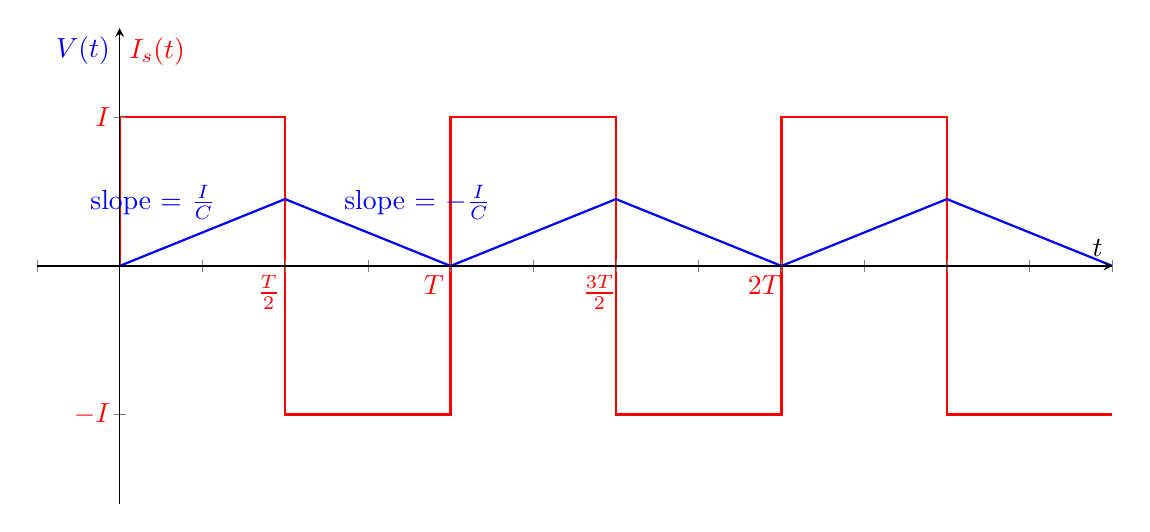
\begin{tikzpicture}
                	\begin{axis}[
                	xmin=-5, xmax=60,
                	ymin=-160, ymax=160,
                	axis lines=center,
                	axis on top=true,
                	grid style={dashed},
                	xlabel={\emph{$t$}},
                	ylabel={\color{red}{\emph{$I_s(t)$}}},
                	yticklabels={,,},
                	xticklabels={,,},
                	width=6in,
                	height=3in,
                	]
                	\addplot [draw=red,thick] coordinates {(0, 0) 
                		(0, 100) (10, 100)
                		(10, -100) (20, -100)
                		(20, 100) (30, 100)
                		(30, -100) (40, -100)
                		(40, 100) (50, 100)
                		(50, -100) (60, -100)};
                	\node [left,color=red] at (axis cs:  0, 100) {$I$}; 
                	\node [left,color=red] at (axis cs:  0, -100) {$-I$}; 
                	\node [below,color=red] at (axis cs:  19, 0) {$T$};
                	\node [below,color=red] at (axis cs:  9, 0) {$\frac{T}{2}$};
                	\node [below,color=red] at (axis cs:  39, 0) {$2T$}; 
                	\node [below,color=red] at (axis cs:  29, 0) {$\frac{3T}{2}$};
                	% voltage
                	\node[left, color=blue] at (axis cs: 0, 145) {$V(t)$};
                	\addplot [draw=blue,thick] coordinates{ (0,0) (10, 45) (20, 0)(30, 45)(40, 0)(50, 45)(60, 0)};
                	\node [above, color=blue] at (axis cs: 2, 25) {slope = $\frac{I}{C}$};
                	\node [above, color=blue] at (axis cs: 18, 25) {slope = $-\frac{I}{C}$};
                	%\node [above, color=blue] at (axis cs: 10,50) {$V = \frac{IT}{2C}$};
                	\end{axis}
            	\end{tikzpicture}
            \end{center}
        }
    \item In parallel with an independent DC current source.
    
        \sol{
            This is similar to the last one, but instead of having negative current sometime, we have a constant positive current throughout the time. As you expected, the voltage will go infinite.
            
            \begin{center}
            	\begin{tikzpicture}
                	\begin{axis}[
                	xmin=-5, xmax=60,
                	ymin=-160, ymax=300,
                	axis lines=center,
                	axis on top=true,
                	grid style={dashed},
                	xlabel={\emph{$t$}},
                	ylabel={\color{red}{\emph{$I_s(t)$}}},
                	yticklabels={,,},
                	xticklabels={,,},
                	width=6in,
                	height=3in,
                	]
                	\addplot [draw=red,thick] coordinates { 
                		(0, 100) (60, 100)
                		};
                	\node [left,color=red] at (axis cs:  0, 100) {$I$}; 
                	\node [left,color=red] at (axis cs:  0, -100) {$-I$}; 
                	\node [below,color=red] at (axis cs:  19, 0) {$T$};
                	\node [below,color=red] at (axis cs:  9, 0) {$\frac{T}{2}$};
                	\node [below,color=red] at (axis cs:  39, 0) {$2T$}; 
                	\node [below,color=red] at (axis cs:  29, 0) {$\frac{3T}{2}$};
                	% voltage
                	\node[left, color=blue] at (axis cs: 0, 145) {$V(t)$};
                	\addplot [draw=blue,thick] coordinates{ (0,0) (60, 270)};
                	\node [above, color=blue] at (axis cs: 2, 25) {slope = $\frac{I}{C}$};
                	%\node [above, color=blue] at (axis cs: 18, 25) {slope = $-\frac{I}{C}$};
                	%\node [above, color=blue] at (axis cs: 10,50) {$V = \frac{IT}{2C}$};
                	\end{axis}
            	\end{tikzpicture}
            \end{center}
        }
    
    
    \item In series with an independent AC sine-wave voltage source in a period of T.
    
        \sol{
            
            Recall the voltage and current's equation of capacitor $I = C\frac{dV}{dt}$, when we take the derivative of voltage equation (sine wave) for current, current becomes a cosine wave on the plot.
            
            \begin{center}
            	\begin{tikzpicture}
                	\begin{axis}[
                	xmin=-5, xmax=60,
                	ymin=-160, ymax=160,
                	axis lines=center,
                	axis on top=true,
                	grid style={dashed},
                	xlabel={\emph{$t$}},
                	ylabel={\color{blue}{\emph{$V(t)$}}},
                	yticklabels={,,},
                	xticklabels={,,},
                	width=6in,
                	height=3in,
                	]
                	% voltage
                	\draw[thick, blue] (50,160) sin (75,260) cos (100,160) sin (125,60) cos (150,160) sin (175,260) cos (200,160) sin (225, 60) cos (250, 160) sin (275, 260) cos (300,160) sin (325, 60) cos (350,160) sin (375,260) cos (400,160) sin (425,60) cos (450,160) sin (475,260) cos (500,160) sin (525, 60) cos (550, 160) sin (575, 260) cos (600, 160) sin (625, 60);
                	
                	\node [left,color=blue] at (axis cs:  0, 100) {$V$}; 
                	\node [left,color=blue] at (axis cs:  0, -100) {$-V$}; 
                	\node [below,color=blue] at (axis cs:  19, 0) {$T$};
                	\node [below,color=blue] at (axis cs:  9, 0) {$\frac{T}{2}$};
                	\node [below,color=blue] at (axis cs:  39, 0) {$2T$}; 
                	\node [below,color=blue] at (axis cs:  29, 0) {$\frac{3T}{2}$};
                	% current
                	\node[left, color=red] at (axis cs: 0, 145) {$I_s(t)$};
                	\draw[thick, red] (50,260) cos (75,160) sin (100,60) cos (125,160) sin (150,260) cos (175,160) sin (200,60) cos (225, 160) sin (250, 260) cos (275, 160) sin (300,60) cos (325, 160) sin (350,260) cos (375,160) sin (400,60) cos (425,160) sin (450,260) cos (475,160) sin (500,60) cos (525, 160) sin (550, 260) cos (575, 160) sin (600, 60) cos (625, 160);
                	%\node [above, color=blue] at (axis cs: 10,50) {$V = \frac{IT}{2C}$};
                	\end{axis}
            	\end{tikzpicture}
            \end{center}
        }
        
    \item In series with an independent DC voltage source.
    
        \sol{
            The key here is still how familiar you are with the equation $I = C\frac{dV}{dt}$. Instead of periodic equation for voltage, now the voltage is constant. When you take the derivative of that for current, the current becomes zero.
        
            \begin{center}
            	\begin{tikzpicture}
                	\begin{axis}[
                	xmin=-5, xmax=60,
                	ymin=-160, ymax=160,
                	axis lines=center,
                	axis on top=true,
                	grid style={dashed},
                	xlabel={\emph{$t$}},
                	ylabel={\color{blue}{\emph{$V(t)$}}},
                	yticklabels={,,},
                	xticklabels={,,},
                	width=6in,
                	height=3in,
                	]
                	% voltage
                	\addplot [draw=blue,thick] coordinates {(0, 100) 
                		(60, 100)};
                	\node [left,color=blue] at (axis cs:  0, 100) {$V$}; 
                	\node [left,color=blue] at (axis cs:  0, -100) {$-V$}; 
                	\node [below,color=blue] at (axis cs:  19, 0) {$T$};
                	\node [below,color=blue] at (axis cs:  9, 0) {$\frac{T}{2}$};
                	\node [below,color=blue] at (axis cs:  39, 0) {$2T$}; 
                	\node [below,color=blue] at (axis cs:  29, 0) {$\frac{3T}{2}$};
                	% current
                	\node[left, color=red] at (axis cs: 0, 145) {$I_s(t)$};
                	\addplot [draw=red,thick] coordinates{ (0,0) (60, 0)};
                	%\node [above, color=blue] at (axis cs: 10,50) {$V = \frac{IT}{2C}$};
                	\end{axis}
            	\end{tikzpicture}
            \end{center}
        }
    
\end{enumerate}

\end{qunlist}

\end{document}

